\section{Thực nghiệm K-line (Robustness với số lượng cụm $k$)}

\subsection{Mục tiêu của Thực nghiệm}

Thông thường, chúng ta không biết trước dữ liệu nên chia thành bao nhiêu cụm là tốt nhất. Một thuật toán tốt phải chạy ổn định dù ta chọn $k=2$ hay $k=10$ - độ ``lì đòn'' (Robustness) của thuật toán FairDen khi người dùng thay đổi số lượng cụm $k$.

\subsection{Thiết lập Thực nghiệm}

\textbf{Đối thủ cạnh tranh:}
\begin{itemize}
    \item \textbf{Fairlet (MCF)} và \textbf{Scalable Fair Clustering}: Chỉ hoạt động với thuộc tính nhạy cảm \textbf{nhị phân} (Binary). Nếu thuộc tính có từ 3 giá trị trở lên (Non-binary), các thuật toán này \textbf{không chạy được}.
    \item \textbf{FairDen} và \textbf{FairSC}: Có thể xử lý đa nhóm (Multi-group).
\end{itemize}

\textbf{Cách thực hiện:} Thay đổi $k$ từ 2 đến 10 và đo Balance, DCSI trên tập Adult với:
\begin{itemize}
    \item \textbf{Race} (5 nhóm): Chỉ có FairDen và FairSC tham gia
    \item \textbf{Gender} (2 nhóm): Tất cả các thuật toán đều tham gia
\end{itemize}

\subsection{Kết quả của Tác giả}

Hình trong bài báo gốc cho thấy FairDen đạt Balance cao nhất với thuộc tính đa nhóm (Race), và đạt DCSI tốt nhất khi $k$ nhỏ với thuộc tính nhị phân (Gender).

\begin{figure}[H]
\centering
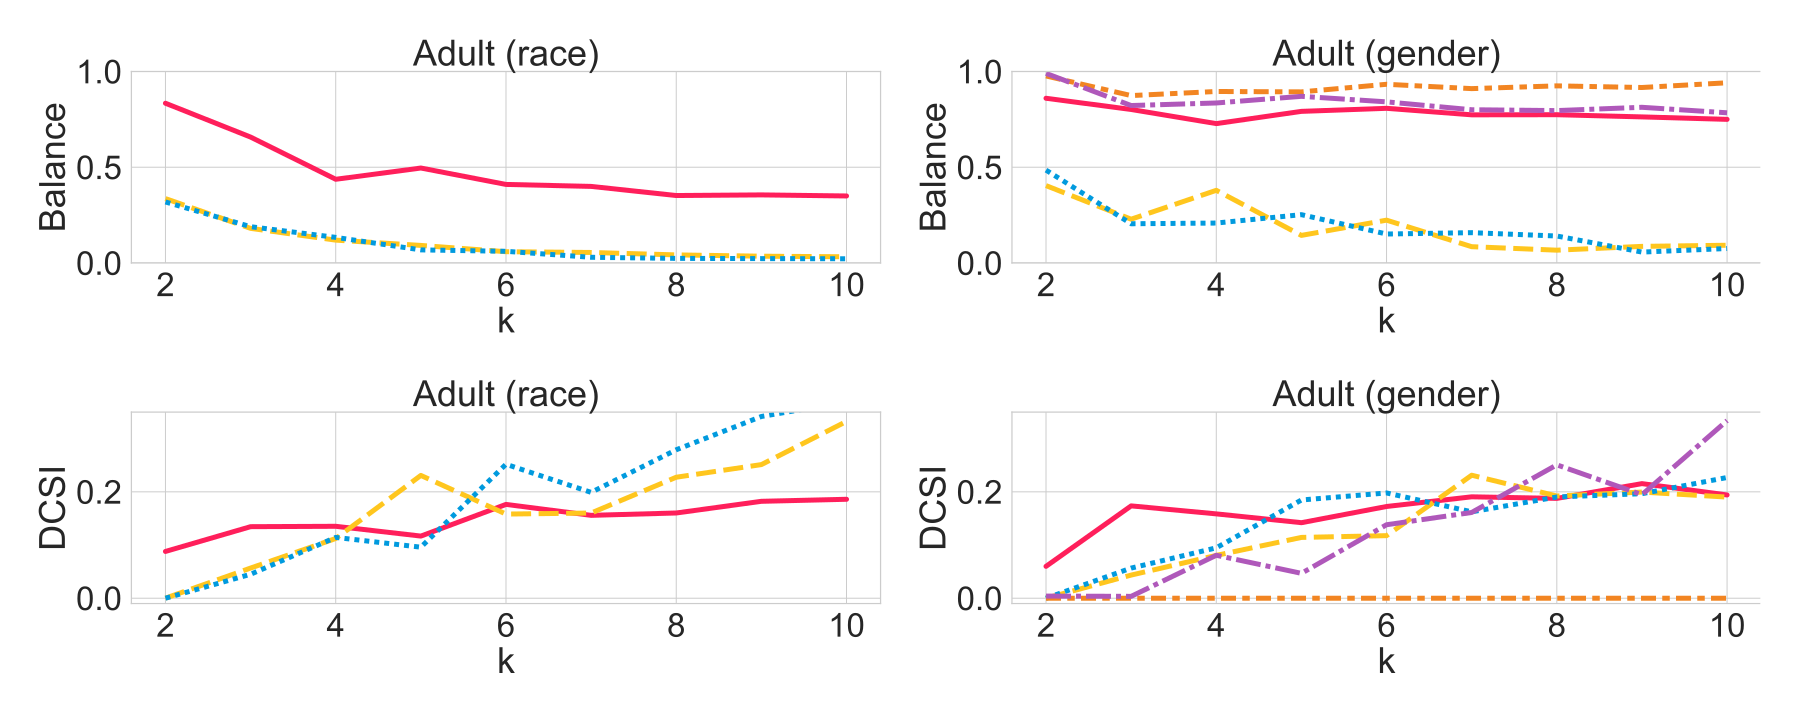
\includegraphics[width=\textwidth]{fig/Lineplot_adult_both.png}
\includegraphics[width=\textwidth]{fig/Legend.png}\\[0.5em]
\caption{Kết quả K-line của tác giả trên tập Adult.}
\label{fig:rw_author}
\end{figure}

\subsection{Kết quả của Nhóm}

\begin{figure}[H]
\centering
\includegraphics[width=\textwidth]{fig/kline_adult_comparison.png}
\caption{Kết quả K-line của nhóm trên tập Adult. Trái: Race (5 nhóm). Phải: Gender (2 nhóm).}
\label{fig:kline_our}
\end{figure}

\textbf{Kết quả trên tập COMPAS (bổ sung của nhóm):}

\begin{figure}[H]
\centering
\includegraphics[width=\textwidth]{fig/kline_compas_comparison.png}
\caption{Kết quả K-line trên tập COMPAS. Trái: Race (4 nhóm). Phải: Sex (2 nhóm).}
\label{fig:kline_compas}
\end{figure}

\subsection{Phân tích Kết quả}

\begin{itemize}
    \item \textbf{Thuộc tính Đa nhóm (Race):} FairDen luôn chiến thắng với Balance cao nhất qua mọi giá trị $k$, cân bằng tỷ lệ các nhóm chủng tộc trong mọi cụm tốt hơn hẳn FairSC. Về chất lượng cấu trúc (DCSI), FairDen đạt mức tương đương với FairSC. Điều này cho thấy FairDen là lựa chọn số 1 cho các bài toán phức tạp có nhiều nhóm nhạy cảm.
    
    \item \textbf{Thuộc tính Nhị phân (Gender/Sex):} Với số cụm nhỏ ($k \leq 5$), FairDen đạt DCSI tốt nhất, giữ được cấu trúc mật độ tốt nhất; với số cụm lớn ($k > 5$), Scalable và FairSC vượt lên một chút do tạo ra các cụm tròn trịa hơn về mặt toán học. Về độ công bằng, hầu hết các phương pháp (FairDen, Scalable, Fairlet) đều đạt Balance cao ($>0.75$), riêng FairSC thường có độ cân bằng thấp hơn.
\end{itemize}

\subsection{Kết luận}

FairDen thể hiện sự đa năng khi là một trong hai thuật toán (cùng FairSC) có thể xử lý dữ liệu phức tạp với thuộc tính nhạy cảm có $\geq 3$ nhóm, đồng thời cho độ công bằng tốt hơn hẳn. Với dữ liệu đơn giản (2 nhóm), FairDen vẫn hoạt động ổn định, đặc biệt khi $k \leq 5$ --- trường hợp phổ biến nhất trong thực tế. Kết quả thực nghiệm của nhóm tái hiện xu hướng trong bài báo gốc, và xu hướng tương tự cũng được quan sát trên tập COMPAS mà nhóm bổ sung thêm.
